\documentclass[brazil,hardcopy,openany,a5paper]{ufscthesis}
\usepackage[brazil]{babel}
\usepackage{amsfonts, amsmath, amsthm, amsbsy,amssymb,bm,mathtools} % For math fonts, symbols and environments %
\usepackage{graphicx} 		% Required for including images
\usepackage{transparent}	% may be required for inkscape pdf figures (http://bit.ly/18i5Oga)
\usepackage{listings}
\usepackage[abnt-emphasize=bf]{abntex2cite}
\usepackage{caption}
\usepackage{multirow}
\usepackage{lscape}
\usepackage[T1]{fontenc}
\sloppy
\usepackage{siunitx}
\usepackage{nameref}
\usepackage{float}

\newcommand{\source}[1]{\small \caption*{Fonte: {#1}} } % Criar fonte embaixo da figura

\newsubfloat{figure}		% Allow subfloats in figure environment (http://bit.ly/1C20NAj)
\graphicspath{{figures/}} 	% Location of the graphics files

\usepackage{siunitx} % units package
\let\DeclareUSUnit\DeclareSIUnit
\let\US\SI
\let\us\si
\DeclareUSUnit\inch{in}
\sisetup{detect-all}  %it may be necessary to load it after loading the font package

\citebrackets[]

%----------------------------------------------------------------------
% Comandos criados pelo usuário
\newcommand{\afazer}[1]{{\color{red}{#1}}} % Para destacar uma parte a ser trabalhada
\DeclareMathOperator*{\argmin}{\arg\!\min}
\DeclareMathOperator*{\argmax}{\arg\!\max}


%----------------------------------------------------------------------
% Identificadores do trabalho
% Usados para preencher os elementos pré-textuais
\instituicao[a]{Universidade Federal de Santa Catarina} % Opcional
\departamento[a]{Biblioteca Universitária}
\programa[o]{Programa de Pós-Graduação em Engenharia Civil} 
\curso{Engenharia de Engenharia Civil}
\documento[a]{Dissertação} % [o] para dissertação e trabalho de conclusão de curso [a] para tese
\grau{Mestre} % doutor, mestre, engenheiro, etc.
\titulo{Modelagem do impacto da ilha de calor sobre o desempenho energético de escritórios condicionados artificialmente}
\subtitulo{} % Opcional
\autor{Marcelo Salles Olinger}
\local{Florianópolis} % Opcional (Florianópolis é o padrão)
\data{24}{junho}{2019}
\orientador[Universidade Federal de Santa Catarina]{Profa. Ana Paula Melo, Dra.}
\coordenador[Universidade Federal de Santa Catariana]{Prof. Fulano de Tal, Dr.}
\orientadornabanca{sim} % Se faz parte da banca definir como sim
\coorientadornabanca{nao} % Se faz parte da banca definir como sim
\bancaMembroA{Prof. Saulo Guths, Dr.\\Universidade Federal de Santa Catarina}  %Nome do presidente da banca
\bancaMembroB{Prof. Membro Dois, Dr.\\Universidade Federal de Santa Catarina}   % Nome do membro da Banca
\bancaMembroC{Profa. Membro Três, Dra.\\Outra Universidade} % Nome do membro da Banca
% \bancaMembroD{Quarto membro\\Universidade ...} % Nome do membro da Banca
% \bancaMembroE{Quinto membro\\Universidade ...}  % Nome do membro da Banca
% \bancaMembroF{Sexto membro\\Universidade ...}   % Nome do membro da Banca
% \bancaMembroG{Sétimo membro\\Universidade ...}  % Nome do membro da Banca

%\dedicatoria{Dedico essa conquista aos amigos e familiares que tornaram isso possível.}

%\agradecimento{Inserir os agradecimentos aos colaboradores à execução do trabalho. Inserir os agradecimentos aos colaboradores à execução do trabalho.}

%\epigrafe{Se você pensa que pode ou se pensa que não pode, de qualquer forma você está certo.}{Henry Ford}

\textoresumo {Texto...}
\palavraschave{Palavra 1. Palavra 2. Palavra 3.}

\textabstract {Text...}
\keywords{Word 1. Word 2. Word 3.}

\begin{document}

	
	%--------------------------------------------------------
	\frontmatter
	% Elementos pré-textuais
	\folhaderosto[pre/Ficha_Catalografica.pdf]
	\folhadeaprovacao{}{} %{pre/signature_page_color.pdf}{}
	%\paginadedicatoria
	%\paginaagradecimento
	%\paginaepigrafe
	\paginaresumo
	\paginaabstract
	% ---
	\listadefiguras % as listas dependem da necessidade do usuário
	\listadetabelas 
	%\listadeabreviaturas
	%\listadesimbolos
	\sumario
	%--------------------------------------------------------
	\mainmatter

	\chapter{Introdução}
	\label{chapter:introducao}
	
	Lorem ipsum dolor sit amet, consectetur adipiscing elit. Nulla commodo, augue non consectetur vehicula, felis velit commodo eros, nec bibendum augue purus quis mi. Donec dapibus id magna eget euismod. In lacinia porttitor velit, in lacinia erat commodo et. Nulla feugiat posuere ipsum, eu euismod lorem efficitur ut. Sed dapibus lobortis ex, eu vehicula sem dignissim nec. Phasellus pellentesque tellus vitae tortor consectetur volutpat. Proin pulvinar lectus id tellus congue maximus \cite{2002boundary}.
	
	Sed semper arcu at posuere scelerisque. Pellentesque a lorem eu lorem lobortis cursus aliquam ut diam. Ut tristique, lacus eget gravida euismod, ante nisl elementum elit, a efficitur neque est eu tellus. Phasellus in convallis tortor. Nullam auctor auctor tempus. Pellentesque placerat, est at convallis congue, velit sapien tempor orci, eu eleifend nisi purus sed odio. Duis nec rhoncus enim. Nunc vitae consectetur sapien. Nullam in enim iaculis, laoreet ex in, aliquet massa. Nulla facilisi. Sed vulputate eros et mi imperdiet, nec commodo libero tristique. Mauris vel pretium felis. Suspendisse feugiat tortor vitae dapibus semper. Fusce dignissim est eget mattis auctor.
	
	Segundo \citeauthoronline{Chen2013} \cite{Chen2013} aenean ultrices feugiat faucibus. Sed ut vehicula ligula, vitae pulvinar enim. Ut vel consectetur dolor, a eleifend mauris. Pellentesque tristique justo id felis consectetur pulvinar. Phasellus diam felis.
	
	\section{Objetivos}
		\subsection{Objetivo geral}

	Lorem ipsum dolor sit amet, consectetur adipiscing elit. Nulla commodo, augue non consectetur vehicula, felis velit commodo eros, nec bibendum augue purus quis mi. Donec dapibus id magna eget euismod. In lacinia porttitor velit, in lacinia erat commodo et. Nulla feugiat posuere ipsum, eu euismod lorem efficitur ut. Sed dapibus lobortis ex, eu vehicula sem dignissim nec. Phasellus pellentesque tellus vitae tortor consectetur volutpat. Proin pulvinar lectus id tellus congue maximus.
	
		\subsection{Objetivos específicos}
	
	Dentre os objetivos específicos deste trabalho estão:

		\begin{itemize}
			\item Lorem ipsum dolor sit amet, consectetur adipiscing elit;
			\item Lorem ipsum dolor sit amet, consectetur adipiscing elit;
			\item Lorem ipsum dolor sit amet, consectetur adipiscing elit;
		\end{itemize}
	
	\section{Estrutura do trabalho}
	
	Lorem ipsum dolor sit amet, consectetur adipiscing elit. Nulla commodo, augue non consectetur vehicula, felis velit commodo eros, nec bibendum augue purus quis mi. Donec dapibus id magna eget euismod. In lacinia porttitor velit, in lacinia erat commodo et. Nulla feugiat posuere ipsum, eu euismod lorem efficitur ut. Sed dapibus lobortis ex, eu vehicula sem dignissim nec. Phasellus pellentesque tellus vitae tortor consectetur volutpat. Proin pulvinar lectus id tellus congue maximus.

	Sed semper arcu at posuere scelerisque. Pellentesque a lorem eu lorem lobortis cursus aliquam ut diam. Ut tristique, lacus eget gravida euismod, ante nisl elementum elit, a efficitur neque est eu tellus. Phasellus in convallis tortor. Nullam auctor auctor tempus. Pellentesque placerat, est at convallis congue, velit sapien tempor orci, eu eleifend nisi purus sed odio. Duis nec rhoncus enim. Nunc vitae consectetur sapien. Nullam in enim iaculis, laoreet ex in, aliquet massa. Nulla facilisi. Sed vulputate eros et mi imperdiet, nec commodo libero tristique. Mauris vel pretium felis. Suspendisse feugiat tortor vitae dapibus semper. Fusce dignissim est eget mattis auctor.

\chapter{Revisão de literatura}
	
	Lorem ipsum dolor sit amet, consectetur adipiscing elit. Nulla commodo, augue non consectetur vehicula, felis velit commodo eros, nec bibendum augue purus quis mi. Donec dapibus id magna eget euismod. In lacinia porttitor velit, in lacinia erat commodo et. Nulla feugiat posuere ipsum, eu euismod lorem efficitur ut. Sed dapibus lobortis ex, eu vehicula sem dignissim nec. Phasellus pellentesque tellus vitae tortor consectetur volutpat. Proin pulvinar lectus id tellus congue maximus.
	
	
	\section{Climatologia}
	
	Lorem ipsum dolor sit amet, consectetur adipiscing elit. Nulla commodo, augue non consectetur vehicula, felis velit commodo eros, nec bibendum augue purus quis mi. Donec dapibus id magna eget euismod. In lacinia porttitor velit, in lacinia erat commodo et. Nulla feugiat posuere ipsum, eu euismod lorem efficitur ut. Sed dapibus lobortis ex, eu vehicula sem dignissim nec. Phasellus pellentesque tellus vitae tortor consectetur volutpat. Proin pulvinar lectus id tellus congue maximus.

	Sed semper arcu at posuere scelerisque. Pellentesque a lorem eu lorem lobortis cursus aliquam ut diam. Ut tristique, lacus eget gravida euismod, ante nisl elementum elit, a efficitur neque est eu tellus. Phasellus in convallis tortor. Nullam auctor auctor tempus. Pellentesque placerat, est at convallis congue, velit sapien tempor orci, eu eleifend nisi purus sed odio. Duis nec rhoncus enim. Nunc vitae consectetur sapien. Nullam in enim iaculis, laoreet ex in, aliquet massa. Nulla facilisi. Sed vulputate eros et mi imperdiet, nec commodo libero tristique. Mauris vel pretium felis. Suspendisse feugiat tortor vitae dapibus semper. Fusce dignissim est eget mattis auctor.
	
		\chapter{Metodologia}
		\label{chapter:metodologia}

	Lorem ipsum dolor sit amet, consectetur adipiscing elit. Nulla commodo, augue non consectetur vehicula, felis velit commodo eros, nec bibendum augue purus quis mi. Donec dapibus id magna eget euismod. In lacinia porttitor velit, in lacinia erat commodo et. Nulla feugiat posuere ipsum, eu euismod lorem efficitur ut. Sed dapibus lobortis ex, eu vehicula sem dignissim nec. Phasellus pellentesque tellus vitae tortor consectetur volutpat. Proin pulvinar lectus id tellus congue maximus.

	Sed semper arcu at posuere scelerisque. Pellentesque a lorem eu lorem lobortis cursus aliquam ut diam. Ut tristique, lacus eget gravida euismod, ante nisl elementum elit, a efficitur neque est eu tellus. Phasellus in convallis tortor. Nullam auctor auctor tempus. Pellentesque placerat, est at convallis congue, velit sapien tempor orci, eu eleifend nisi purus sed odio. Duis nec rhoncus enim. Nunc vitae consectetur sapien. Nullam in enim iaculis, laoreet ex in, aliquet massa. Nulla facilisi. Sed vulputate eros et mi imperdiet, nec commodo libero tristique. Mauris vel pretium felis. Suspendisse feugiat tortor vitae dapibus semper. Fusce dignissim est eget mattis auctor.

	Aenean ultrices feugiat faucibus. Sed ut vehicula ligula, vitae pulvinar enim. Ut vel consectetur dolor, a eleifend mauris. Pellentesque tristique justo id felis consectetur pulvinar. Phasellus diam felis.

\begin{table}[!h]
	\centering
	\caption{Figura 1}
	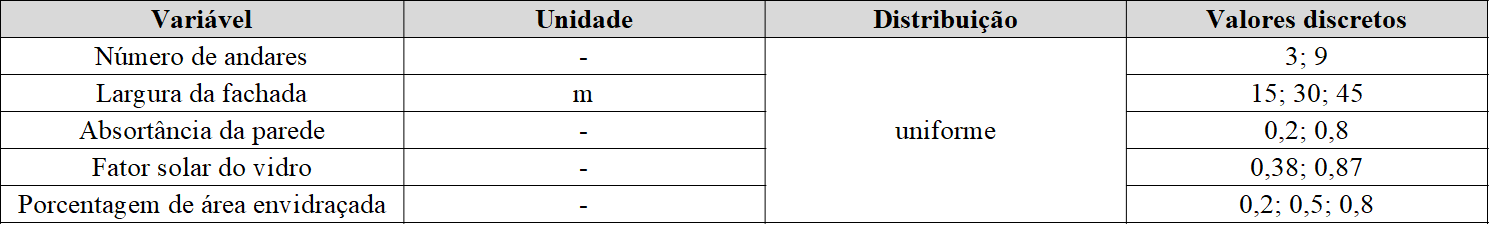
\includegraphics[width=1\linewidth]{img/tabelaedificacao.png}
	\label{table:tabelaedificacao}
\end{table}

	Lorem ipsum dolor sit amet, consectetur adipiscing elit. Nulla commodo, augue non consectetur vehicula, felis velit commodo eros, nec bibendum augue purus quis mi. Donec dapibus id magna eget euismod. In lacinia porttitor velit, in lacinia erat commodo et. Nulla feugiat posuere ipsum, eu euismod lorem efficitur ut. Sed dapibus lobortis ex, eu vehicula sem dignissim nec. Phasellus pellentesque tellus vitae tortor consectetur volutpat. Proin pulvinar lectus id tellus congue maximus.

Sed semper arcu at posuere scelerisque. Pellentesque a lorem eu lorem lobortis cursus aliquam ut diam. Ut tristique, lacus eget gravida euismod, ante nisl elementum elit, a efficitur neque est eu tellus. Phasellus in convallis tortor. Nullam auctor auctor tempus. Pellentesque placerat, est at convallis congue, velit sapien tempor orci, eu eleifend nisi purus sed odio. Duis nec rhoncus enim. Nunc vitae consectetur sapien. Nullam in enim iaculis, laoreet ex in, aliquet massa. Nulla facilisi. Sed vulputate eros et mi imperdiet, nec commodo libero tristique. Mauris vel pretium felis. Suspendisse feugiat tortor vitae dapibus semper. Fusce dignissim est eget mattis auctor.

Aenean ultrices feugiat faucibus. Sed ut vehicula ligula, vitae pulvinar enim. Ut vel consectetur dolor, a eleifend mauris. Pellentesque tristique justo id felis consectetur pulvinar. Phasellus diam felis.

\begin{equation}
	\label{eq:variacaopercentual}
	VariacaoPercentual_{i} = 100 \cdot \frac{MetodoModelagem_{i}}{RSCP} - 100
\end{equation}

Lorem ipsum dolor sit amet, consectetur adipiscing elit. Nulla commodo, augue non consectetur vehicula, felis velit commodo eros, nec bibendum augue purus quis mi. Donec dapibus id magna eget euismod. In lacinia porttitor velit, in lacinia erat commodo et. Nulla feugiat posuere ipsum, eu euismod lorem efficitur ut. Sed dapibus lobortis ex, eu vehicula sem dignissim nec. Phasellus pellentesque tellus vitae tortor consectetur volutpat. Proin pulvinar lectus id tellus congue maximus.

Sed semper arcu at posuere scelerisque. Pellentesque a lorem eu lorem lobortis cursus aliquam ut diam. Ut tristique, lacus eget gravida euismod, ante nisl elementum elit, a efficitur neque est eu tellus. Phasellus in convallis tortor. Nullam auctor auctor tempus. Pellentesque placerat, est at convallis congue, velit sapien tempor orci, eu eleifend nisi purus sed odio. Duis nec rhoncus enim. Nunc vitae consectetur sapien. Nullam in enim iaculis, laoreet ex in, aliquet massa. Nulla facilisi. Sed vulputate eros et mi imperdiet, nec commodo libero tristique. Mauris vel pretium felis. Suspendisse feugiat tortor vitae dapibus semper. Fusce dignissim est eget mattis auctor.

Aenean ultrices feugiat faucibus. Sed ut vehicula ligula, vitae pulvinar enim. Ut vel consectetur dolor, a eleifend mauris. Pellentesque tristique justo id felis consectetur pulvinar. Phasellus diam felis.

\chapter{Resultados e Discussões}
\label{chapter:resultados}

Lorem ipsum dolor sit amet, consectetur adipiscing elit. Nulla commodo, augue non consectetur vehicula, felis velit commodo eros, nec bibendum augue purus quis mi. Donec dapibus id magna eget euismod. In lacinia porttitor velit, in lacinia erat commodo et. Nulla feugiat posuere ipsum, eu euismod lorem efficitur ut. Sed dapibus lobortis ex, eu vehicula sem dignissim nec. Phasellus pellentesque tellus vitae tortor consectetur volutpat. Proin pulvinar lectus id tellus congue maximus.

Sed semper arcu at posuere scelerisque. Pellentesque a lorem eu lorem lobortis cursus aliquam ut diam. Ut tristique, lacus eget gravida euismod, ante nisl elementum elit, a efficitur neque est eu tellus. Phasellus in convallis tortor. Nullam auctor auctor tempus. Pellentesque placerat, est at convallis congue, velit sapien tempor orci, eu eleifend nisi purus sed odio. Duis nec rhoncus enim. Nunc vitae consectetur sapien. Nullam in enim iaculis, laoreet ex in, aliquet massa. Nulla facilisi. Sed vulputate eros et mi imperdiet, nec commodo libero tristique. Mauris vel pretium felis. Suspendisse feugiat tortor vitae dapibus semper. Fusce dignissim est eget mattis auctor.

Aenean ultrices feugiat faucibus. Sed ut vehicula ligula, vitae pulvinar enim. Ut vel consectetur dolor, a eleifend mauris. Pellentesque tristique justo id felis consectetur pulvinar. Phasellus diam felis.

\chapter{Conclusões}
\label{chapter:conclusoes}
	
Lorem ipsum dolor sit amet, consectetur adipiscing elit. Nulla commodo, augue non consectetur vehicula, felis velit commodo eros, nec bibendum augue purus quis mi. Donec dapibus id magna eget euismod. In lacinia porttitor velit, in lacinia erat commodo et. Nulla feugiat posuere ipsum, eu euismod lorem efficitur ut. Sed dapibus lobortis ex, eu vehicula sem dignissim nec. Phasellus pellentesque tellus vitae tortor consectetur volutpat. Proin pulvinar lectus id tellus congue maximus.

Sed semper arcu at posuere scelerisque. Pellentesque a lorem eu lorem lobortis cursus aliquam ut diam. Ut tristique, lacus eget gravida euismod, ante nisl elementum elit, a efficitur neque est eu tellus. Phasellus in convallis tortor. Nullam auctor auctor tempus. Pellentesque placerat, est at convallis congue, velit sapien tempor orci, eu eleifend nisi purus sed odio. Duis nec rhoncus enim. Nunc vitae consectetur sapien. Nullam in enim iaculis, laoreet ex in, aliquet massa. Nulla facilisi. Sed vulputate eros et mi imperdiet, nec commodo libero tristique. Mauris vel pretium felis. Suspendisse feugiat tortor vitae dapibus semper. Fusce dignissim est eget mattis auctor.

Aenean ultrices feugiat faucibus. Sed ut vehicula ligula, vitae pulvinar enim. Ut vel consectetur dolor, a eleifend mauris. Pellentesque tristique justo id felis consectetur pulvinar. Phasellus diam felis.


\section{Limitações e justificativas}

As limitações desse estudo são indicadas em conformidade com a ordem de execução das etapas de desenvolvimento:

\begin{itemize}
	\item Lorem ipsum dolor sit amet, consectetur adipiscing elit. Nulla commodo, augue non consectetur vehicula, felis velit commodo eros, nec bibendum augue purus quis mi. Donec dapibus id magna eget euismod;
	
	\item Lorem ipsum dolor sit amet, consectetur adipiscing elit. Nulla commodo, augue non consectetur vehicula, felis velit commodo eros, nec bibendum augue purus quis mi. Donec dapibus id magna eget euismod;
	
	\item Lorem ipsum dolor sit amet, consectetur adipiscing elit. Nulla commodo, augue non consectetur vehicula, felis velit commodo eros, nec bibendum augue purus quis mi. Donec dapibus id magna eget euismod.
	
\end{itemize}

\section{Sugestões para trabalhos futuros}

As sugestões para trabalhos futuros são indicadas em conformidade com as potencialidades expressas nesse estudo, sendo:

\begin{itemize}
	\item Lorem ipsum dolor sit amet, consectetur adipiscing elit. Nulla commodo, augue non consectetur vehicula, felis velit commodo eros, nec bibendum augue purus quis mi. Donec dapibus id magna eget euismod;

	\item Lorem ipsum dolor sit amet, consectetur adipiscing elit. Nulla commodo, augue non consectetur vehicula, felis velit commodo eros, nec bibendum augue purus quis mi. Donec dapibus id magna eget euismod;

	\item Lorem ipsum dolor sit amet, consectetur adipiscing elit. Nulla commodo, augue non consectetur vehicula, felis velit commodo eros, nec bibendum augue purus quis mi. Donec dapibus id magna eget euismod.
	
\end{itemize}

\begin{appendices}
	\chapter{Classificação climática de Köppen-Geiger}
	\begin{figure}[!h]
		\centering
		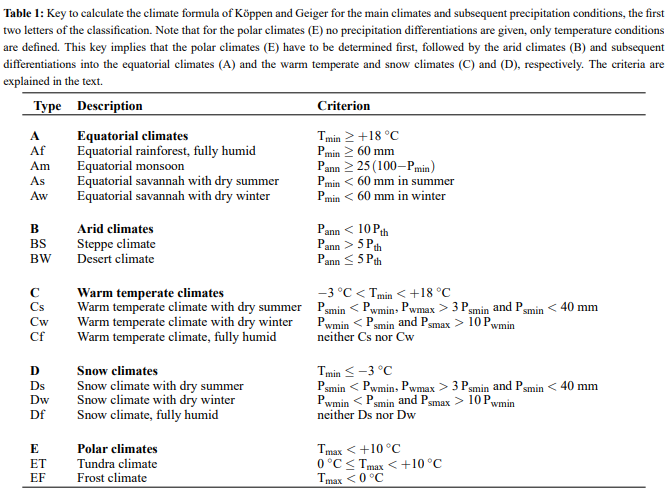
\includegraphics[width=1\linewidth]{img/tablekoppengeiger1.png}
		\label{fig:tablekoppengeiger1}
	\end{figure}
\end{appendices}

\begin{appendices}
	\chapter{Código...}
	\lstset{language=c++}
	\lstset{label={lst:code_direct}}
	\lstset{basicstyle=\tiny}	
	\lstinputlisting{code/code.cc}
\end{appendices}

%\bibliographystyle{lib/abntex2-num}
%\bibliographystyle{lib/abntex2-alf}
\bibliography{citacoes}
	
\end{document}